\documentclass[conference]{IEEEtran}
\usepackage{graphicx}    % needed for including graphics e.g. EPS, P
\usepackage[pdftex]{hyperref}
\usepackage{listings}
\lstset{language=C}
\usepackage{url}
\begin{document}
\title{YANG Language Parser for Libsmi}
\author{\IEEEauthorblockN{Siarhei Kuryla}
\IEEEauthorblockA{Jacobs University Bremen\\
Spring Semester 2009\\
Supervisor: Prof. Dr. Juergen Schoenwaelder}
}

% make the title area
\maketitle

\begin{abstract}
NETCONF is a network management protocol developed in the IETF by the Netconf working group  which provides a simple mechanism through which a network device can be managed, configuration data information can be retrieved, and new configuration data can be uploaded and manipulated. YANG is a data modeling language used to model configuration and state data manipulated by the NETCONF protocol, NETCONF remote procedure calls, and NETCONF notifications. The YANG language is currently being developed by the IETF NETCONF Data Modeling Language Working Group. The libsmi is a library which provides a C API to access network management data model definitions written in various versions of the SMI (Structure of Management Information). The goal of this project is to extend a libsmi parser for the YANG data modeling language in order to make it compliant with the latest version of the YANG language.
\end{abstract}

\section{Introduction}
YANG is a data modeling language used to model configuration and state data manipulated by the NETCONF protocol, NETCONF remote procedure calls, and NETCONF notifications. Today, the NETCONF protocol \cite{bib1} lacks a standardized way to create data models. Instead, vendors are forced to use proprietary solutions. In order for NETCONF to be a interoperable protocol, models must be defined in a vendor-neutral way. YANG provides the language and rules for defining such models for use with NETCONF. 

YANG is posed as simple and easy to learn because of its trivial and regular syntax. This language is NETCONF-specific language designed to do what it needs to do well and it does not try to compete with XSD. YANG is fully modular and it enables development of certain parts of the model without influencing those parts that need no change. The YANG language is still under development and the latest draft version of this language was released on April 20, 2009 

Libsmi is a C library which provides a convenient API for handling network management data model definitions written in various versions of the SMI. The project's main task is to create a YANG parser for the library, update it's inner data structures to support the new language, and extend the API to support the new features of the YANG language.

\section{Motivation and problem statement}
The YANG language is still being developed and it is not yet widely used. Availability of convenient programming tools which support this modeling language might facilitate its adoption. Libsmi is  a portable C library that currently provides an API for access to various versions of the SMI. This library hides parsing details providing accessing SMI definitions for applications. Libsmi is a potential tool to be extended to support the YANG language. 

When I was starting working on the project there was already an incomplete parser implementation for libsmi based on the early version of the YANG specification  \cite{bib2}. The implementation was incomplete and suffered from a number of problems: 
\begin{itemize}
	\item the lexical analyzer was implemented inaccurately. There were various problems with qoutings, line counting, string concatenation and some general rules were defined wrong;
	\item the syntactic analyzer was implemented inaccurately. The implementation did not cover the whole grammar of the YANG language and there were many collisions with the specification;
	\item the implementation was incomplete: some language statements were stored to internal data structures, others were not;
	\item the implementation tried to retrofit the YANG data model into existing libsmi data structures and API functions. However it caused many problems, making the parser much more complicated. It was confusing what functions we should use to handle a particular language definition, what data structure and members of the data structure correspond to the definition;
	\item there was no semantic analysis. References to groupings, types, features, and identities were not resolved, uniqueness of identifiers was not validated, modules knew nothing about definitions in their submodules.
\end{itemize}

This project aims at completing the parser for the YANG data modeling language in order to make it compliant with the latest version of the YANG language. At the time when the project was starting the available version of the specification was draft-ietf-netmod-yang-03 \cite{bib3} and it is used as a basis for the entire project.

%\section{YANG language concepts}
%The base unit of definition in YANG is a module, which defines a single data model. A module might be partitioned into a number of submodules that contribute definitions to the module. One module might refer other modules' definitions importing them. 

\section{Libsmi library}
The core of the libsmi library allows management applications to access SMI MIB module definitions. 
The structure of the library \cite{bib7} is internally divided into two layers. 
The upper layer provides the API to applications that make use of libsmi and internal data structures to management information in memory. 
The lower layer is a collection of drivers (actual parsers) that retrieve the management information from the SMI definitions.
The details of the libsmi architecture are illustrated in the figure \ref{fig:libsmi}.  

The libsmi library distribution also includes a collection of tools built on top of the library to check, analyze dump, convert, and compare MIB definitions.

In order to support a new modeling language by the libsmi library a driver for this language has to be implemented (a parser for the language), the way how to store language definitions in memory has to be specified by reusing already available data structures or implementing new ones, and the API to access module definitions has to be exposed. In order to be able to serialize module definitions stored in memory the smidump tool might be used which requites to implement a driver that defines serialization rules.
\begin{figure}
\begin{center}
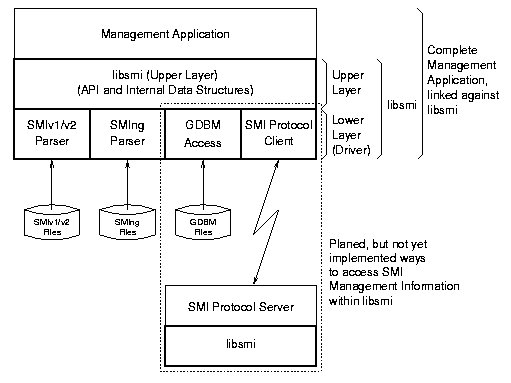
\includegraphics[scale=0.50]{libsmi.jpg}
\caption{ Libsmi architecture}
\label{fig:libsmi}
\end{center}
\end{figure}

\section{YANG module parsing}
The parsing of a YANG module is accomplished over several phases, which includes lexical, syntactic and semantic analysis.
\subsection{Lexical analysis}
Lexical analysis allows to convert an input sequence of characters into a sequence of tokens which are atomic language units such as keywords, identifiers, text segment and number definitions. A lexical analyzer processes the input characters to categorize them according to function, giving them meaning.

In the project lexical analysis is done by the lexical analyzer which is generated by the flex tool \cite{bib5}. The flex program reads a description of a lexical analyzer to generate from the given input file. The description is in the form of pairs of regular expressions and C statements associated with them. Flex generates as output a C source file which is a lexical analyzer for the given description. This output file has to be compiled and linked to produce an executable. When the executable is run, it analyzes its input for occurrences of the regular expressions and once it matches an input character sequence with a regular expression it executes the C code associated with it.

The file \texttt{lib/scanner-yang.l} contains the description of the lexical analyzer for the YANG language. A token in YANG is either a keyword, a string, ";", "\{", or "\}". First of all, regular expressions for all keywords of the YANG language are defined and C statements which return the type of the keyword are associated with them. A string might be either unquoted  or enclosed within double or single quotes depending on the characters the string contains. Identifiers, identifier references (which are in the form prefix:identifier) and dates  are specific kinds of strings. The rules to handle all these kinds of strings are defined in the description of the lexical analyzer. If a quoted string is followed by a plus character ("+"), followed by
 another quoted string, the two strings have to be concatenated which is also accomplished here.

YANG supports two kinds of comments: a single line comment which starts with "//" and  ends at the end of the line; a block comment which is enclosed within "/*"  and "*/". The lexical analyzer contains rules which filter out both kinds of comments from the input character sequence.

Lexical analyzer is also responsible for counting line numbers to associate them with tokens.

\subsection{Syntactic analysis}
Syntactic analysis processes a sequence of tokens obtained from the lexical analysis and determines their grammatical structure with respect to a given formal grammar. In other words, it checks whether it is possible to construct a particular sequence of tokens by applying grammar rules of the language. Apart from the validation for correct syntax the syntactic analysis also builds a parse tree for the input token sequence. 

In order to create a syntactic analyzer for the YANG language bison parser generator \cite{bib6} is used, which is a part of the GNU project. Bison converts a grammar description for a context-free grammar into a C program which can parse a sequence of tokens that conforms to that grammar. 

The file \texttt{lib/parser-yang.y} is a Bison grammar file that contains the grammar of the YANG language in Bison syntax. The first part of this grammar file is Bison declarations where the names of all terminal and nonterminal symbols are declared. The rest of the file implements the YANG ABNF grammar rules defined in the specification. In a Bison grammar, a grammar rule might have an action made up of C statements. Each time the parser recognizes a match for that rule, the action is executed. The associated with the grammar rules C statements accomplish simple validations and construct a representation of the parsing module in memory.

\subsection{Semantic analysis}
When the syntactic analysis is done we know that the YANG module is grammatically correct and we have the representation of the module in internal data structures, but it still does not mean that the  module is valid. Semantic analysis is the phase in which semantic information is added to tree built in the previous phase. This phase performs semantic checks which require a complete module tree. For instance, these are some examples of validations that have to be applied in this phase:
\begin{itemize}
\item resolve all references to user defined types, groupings, extensions, identities and features.
\item check whether there are no
  circular dependencies between various module elements such as user-defined types, groupings, identities, features and modules themselves;
\item check whether all identifiers have unique names in the scope of their namespaces;
\item check whether restrictions applied to user defined types don't create collisions;
\end{itemize}

\section{Data structures}
The output of the syntactic analysis is stored in memory in internal libsmi data structures. The library has two layers of data structures - public and private. The public data structures are exposed through the library API. The private data structures are used only inside the library itself and contain the corresponding public data structures, as well as many additional fields which are necessary in the validation phase. 

The libsmi library already contains a set of implemented data structures for other modeling languages. While adding support for the YANG language there were two options:
\begin{itemize}
\item try to retrofit YANG model into existing data structures and APIs;
\item create a separate set of data structures and API functions for YANG from scratch;
\end{itemize}

Each approach has some advantages and disadvantages. In the first case we might keep the API of the library unchanged and, theoretically, the applications that use the libsmi library and have been developed before don't require additional changes (or require minor changes). But, practically, it suffers from a number of limitations. The YANG language is pretty different from the languages libsmi supports and it would be not a trivial task to fit the YANG model into existing data structures and APIs. Even though it is doable it would be necessary to modify some existing data structures and add new ones. It results in very complicated data structures some fields of which are used by one modeling language and not used by another one. As a result the development process gets extremely difficult because we have to operate on the data structures we have, but not ones that are best suited. In order to work with the library one should spend much time on learning how  data is actually stored. 

The later approach makes the development and usage of the library much simpler, but it loses the compatibility. We can create data structures which are best suited for the language model. It will also make the API of the library clearer. In order to support the compatibility at the API level it is possible to implement conversion functions which allow to convert a module between different languages. 

In the project the second approach was chosen: all necessary data structures and the public API were defined from scratch.

\subsection{Public data structures}
Public data structures and user defined types for the YANG language are declared in the \texttt{lib/yang.h} file. All of them are named with the \texttt{Yang} prefix. 

The \texttt{YangNode} data structure is used for representing YANG statements of any kind:
\small
\begin{center}
\begin{verbatim}
    typedef struct YangNode {
        YangString      value;
        YangString      extra;
        YangDecl        nodeKind;
        YangStatus      status;
        YangConfig      config;
        YangString      *description;
        YangString      *reference;
    } YangNode;
\end{verbatim}
\end{center}
\normalsize
The \texttt{nodeKind} field of the \texttt{YangDecl} enumerated C type specifies the kind of the YANG statement that corresponds to the node. The \texttt{YangDecl} type declares 65 possible values (e.g. \texttt{YANG\_DECL\_IMPORT}). The \texttt{YANG\_DECL\_UNKNOWN} value represents the statements which are user defined extensions.

The \texttt{value} field of the \texttt{YangString} type holds the argument of the statement.

The \texttt{extra} field of the \texttt{YangString} type is only used by the statements which are user defined extensions with an argument to store the argument.

The \texttt{status} field of the \texttt{YangStatus} type holds the value of the enclosed status statement (if the status is not present then the \texttt{YANG\_STATUS\_DEFAULT\_CURRENT} value).

The \texttt{config} field of the \texttt{YangConfig} type holds the value of the enclosed config statement (if the config is not present then the \texttt{YANG\_CONFIG\_DEFAULT\_CURRENT} value).

The \texttt{description} and \texttt{reference} fields of the \texttt{YangString} type hold the values of the enclosed description and reference statements respectively.

\subsection{Private data structures}
Private data structures are declared in the \texttt{lib/yang-data.h} file and have the \texttt{\_Yang} prefix in their names. 

All YANG module statements are represented in memory by the \texttt{\_YangNode} data structure:
\small
\begin{verbatim}
    typedef struct _YangNode {
        YangNode            export;
        YangNodeType        nodeType;
        void                *info;
        int                 line;
        struct _YangTypeInfo *typeInfo;
        struct _YangNode  	*firstChildPtr;
        struct _YangNode  	*lastChildPtr;    
        struct _YangNode  	*nextSiblingPtr;
        struct _YangNode  	*parentPtr;
        struct _YangNode  	*modulePtr;
    } _YangNode;
\end{verbatim}
\normalsize

The first \texttt{export} field of the \texttt{YangNode} type is a corresponding public data structure of a YANG node which is exposed through the API of the library. This fact allows to cast public data structure pointers to private data structure pointers, e.g.
\small
\begin{verbatim}
_YangNode *nodePtr = (_YangNode*)yangNodePtr
\end{verbatim}
\normalsize
where \texttt{yangNodePtr} is of the \texttt{YangNode} type.

The purpose of the \texttt{nodeType} field of the enumerated \texttt{YangNodeType} type is described later on in this report. All nodes corresponding to the  definitions of the YANG module have \texttt{YANG\_NODE\_ORIGINAL} as the value of this field.

The \texttt{info} pointer is used to  refer additional data structures which hold the information specific for different types of YANG statements. For instance, if the node represents the module statement then the pointer contains the reference to the \texttt{\_YangModuleInfo} data structure.

The \texttt{line} field holds the number of the line in the module file corresponding to the statement which is represented by the node.

The \texttt{typeInfo} field is intended to be used by nodes which represent the typedef statements (to hold a reference to the base type and restrictions applied to the type). At the present the type validations are not implemented, so the field is not used.

The \texttt{\_YangNode} data structure is a list, every element of which has a reference to the next element \texttt{nextSiblingPtr}. 

The \texttt{firstChildPtr}  and \texttt{lastChildPtr} fields hold pointers to the first and last nodes which represent statements enclosed into the current node.

The \texttt{parentPtr}  field holds a pointer to the node that represents the statement which encloses this one.

The \texttt{modulePtr}  field is a reference to the node corresponding to the module statement to which  the current node belongs.

Using the same data structure for representing all YANG statements makes it possible to process all nodes of a module tree in the same way, 
what allows to generalize the logic of many validations and ease the implementation.

\section{YANG public API functions}
At the present the public API for handling YANG module definitions is fairly poor. But all required data is stored in private data structures and later on another view on them might be exposed.

All YANG API functions have the \texttt{yang} prefix and are declared in the \texttt{lib/yang.h} file:
\begin{itemize}
\item 
\small
\begin{verbatim}
int yangIsModule(const char* name)
\end{verbatim}
\normalsize
 returns \texttt{true} if the module with the given name is a YANG module;

\item 
\small
\begin{verbatim}
YangNode *yangGetModule(char *name)
\end{verbatim}
\normalsize
returns a pointer to the struct \texttt{YangNode} for the module with the given name or \texttt{NULL} if the YANG module with the given has not been loaded;

\item 
\small
\begin{verbatim}
YangNode *yangGetFirstModule(void)
\end{verbatim}
\normalsize
returns a pointer to the struct \texttt{YangNode} that represents the first loaded YANG module or \texttt{NULL} if no one YANG module has been loaded;

\item 
\small
\begin{verbatim}
YangNode *yangGetNextModule(
                  YangNode *yangModulePtr)
\end{verbatim}
\normalsize
returns a pointer to the struct \texttt{YangNode} that represents the YANG module loaded after the given module \texttt{yangModulePtr} or \texttt{NULL} if there is no YANG module loaded after it;

\item 
\small
\begin{verbatim}
YangNode *yangGetFirstChildNode(
                    YangNode *yangNodePtr)
\end{verbatim}
\normalsize
returns a pointer to the struct \texttt{YangNode} that represents the first child node of the \texttt{yangNodePtr} node or \texttt{NULL} if that node does have child nodes;

\item 
\small
\begin{verbatim}
YangNode *yangGetNextSibling(
                    YangNode *yangNodePtr)
\end{verbatim}
\normalsize
returns a pointer to the struct \texttt{YangNode} that represents next sibling node of the \texttt{yangNodePtr} node or \texttt{NULL} if there is no next sibling node;

\item 
\small
\begin{verbatim}
int yangIsTrueConf(YangConfig conf)
\end{verbatim}
\normalsize
returns \texttt{1} if the given \texttt{YangConfig} value is true and \texttt{0} otherwise.
\end{itemize}

While working with the YANG API there are several library API functions which still have to be used (for initialization and adjustment operations):
\begin{itemize}
\item 
\small
\begin{verbatim}
int smiInit(const char *tag)
\end{verbatim}
\normalsize
initializes internal data structures;

\item 
\small
\begin{verbatim}
void smiExit(void)
\end{verbatim}
\normalsize
releases allocated resources;

\item 
\small
\begin{verbatim}
char *smiLoadModule(const char *module)
\end{verbatim}
\normalsize
loads a module with the given name in memory;
\end{itemize}

\section{Implementation details}
\subsection{Module loading}
YANG modules are loaded into memory by execution of the function 
\small
\begin{verbatim}
    loadYangModule(const char *modulename, 
                   const char *revision, 
                   Parser *parserPtr),
\end{verbatim}
\normalsize
where the module name must be specified, the revision and pointer to a parser are optional arguments. The \texttt{Parser} data structure declared in the \texttt{lib/data.h} file is used by all language drivers and contains a collection of parsing parameters and flags.

The execution of this function triggers the parsing of the module. While parsing the module, C statements associated with the grammar rules (defined in the Bison grammar description) are executed. These statements create the corresponding node in the module tree for every module definition and apply validations that don't require a complete module representation in memory.

In order to add a new node into the module tree the function
\small
\begin{verbatim}
   _YangNode *addYangNode(const char *value, 
                          YangDecl nodeKind, 
                          _YangNode *parentPtr)
\end{verbatim}
\normalsize
is used.
The first parameter \texttt{value} of the function is the argument of the YANG statement (e.g., the name of the module for the module statement, an XPath expression for the must, when and augment statements). The second parameter represents the kind of the YANG statement that corresponds to the created node. And the last argument is a pointer to the parent node.

For some module tree nodes the \texttt{info} field of the \texttt{\_YangNode} data structure is initialized here. What data is stored in this field depends on the the type of the YANG statement:
\subsubsection{"module" and "submodule" statements}
the \texttt{info} field refers to the \texttt{\_YangModuleInfo} data structure:

\small
\begin{verbatim}
   typedef struct _YangModuleInfo {
       char              *prefix;
       char              *version;
       char              *namespace;
       char              *organization;
       char              *contact;
       _YangParsingState parsingState;
       struct _YangNode  *originalModule;
       struct YangList   *submodules;
       struct YangList   *imports;
       void              *parser;
} _YangModuleInfo;
\end{verbatim}
\normalsize
The \texttt{prefix}, \texttt{namespace}, \texttt{organization} and \texttt{contact} fields hold the arguments of the prefix, namespace, organization and contact statements enclosed into the module or submodule. The \texttt{version} field contains the specified version of the YANG language.

The \texttt{parsingState} field of the enumerated \texttt{\_YangParsingState} type represents the parsing state of the module and contains one of the following values:
\begin{itemize}
\item \texttt{YANG\_PARSING\_IN\_PROGRESS} - the module is currently being parsed;
\item \texttt{YANG\_PARSING\_DONE} - parsing of the module has already been finished;
\end{itemize}
This field is used to be able to determine circular dependencies between modules and submodules.

The purpose of the \texttt{originalModule} field is explained later in this document.

The \texttt{submodules} and \texttt{imports} fields are linked lists of pointers to included submodules and imported modules respectively (YANG list data structures are examined later in this section).

\subsubsection{"if-feature", "typedef", "uses", "base" statements and user-defined extensions}
the \texttt{info} field refers to the \texttt{\_YangIdentifierRefInfo} data structure:
\small
\begin{verbatim}
    typedef struct _YangIdentifierRefInfo {
        char        *prefix;
        char        *identifierName;
        _YangNode   *resolvedNode;
        _YangNode   *marker;
    } _YangIdentifierRefInfo;
\end{verbatim}
\normalsize
Everyone of these statements takes an identifier reference as an argument. An identifier reference consists of the prefix of the module (which might be omitted if one refers the element in the current module) and the identifier, which are stored in the \texttt{prefix} and \texttt{identifierName} fields respectively. The field \texttt{resolvedNode} is a pointer to the node in the current or imported module which corresponds to the identifier reference. The \texttt{marker} field is used to detect circular dependencies between module elements.

\subsubsection{"grouping" statement}
the \texttt{info} field refers to the \texttt{\_YangGroupingInfo} data structure:
\small
\begin{verbatim}
    typedef struct _YangGroupingInfo {
        _YangParsingState state;
    } _YangGroupingInfo;
\end{verbatim}
\normalsize
This data structure contains only one field, which represents the parsing state of the grouping definition and is used in circular dependency detection.

\subsubsection{"key" and "unique" statements}
These statements take as an argument a string which contains a space separated list of node identifier references. The \texttt{info} field holds a parsed list of identifier references.

\subsection{Importing and including modules}
YANG allows to specify the revision of the imported module or included submodule. When a module is published, it uses the current available revisions of other modules. Publishing new revisions of the imported modules  does not affect the importing module, since it still uses revisions which have been published before. This YANG mechanism allows modules to evolve independently over time. 

According to the specification, YANG modules and submodules are typically stored in files, one module or submodule per file, and the name of the file should be on the form:
\small
\begin{verbatim}
(sub)module-name ['.' revision-date] ('.yang')
\end{verbatim}
\normalsize

When the import (include) statement is encountered in the parsing module, the corresponding module (submodule) is loaded into memory by 
\small
\begin{verbatim}
_YangNode *externalModule(_YangNode *importNode);
\end{verbatim}
\normalsize
function invocation. If a revision for the imported module is present then the implementation tries to load a module with the specified revision. 
If such module has not been found, the library attempts to load a module with no revision.
While loading imported modules (submodules) there is validation that allows to detect circular dependencies between them.

\subsection{Private API functions}
Private API functions are defined in the \texttt{lib/yang-data.h} file. 
Some of them have been already mentioned and explained in the previous sections. Here is a list of primary private API functions:
\begin{itemize}
\item
\small
\begin{verbatim}
_YangNode *loadYangModule(
                   const char *modulename, 
                   const char * revision, 
                   Parser *parserPtr)
\end{verbatim}
\normalsize

loads a module with by the given name and revision.
\item
\small
\begin{verbatim}
void yangFreeData()
\end{verbatim}
\normalsize
frees the memory allocated for all loaded YANG modules. 

\item
\small
\begin{verbatim}
YangNode *findYangModuleByName(
   const char *modulename, char* revision)
\end{verbatim}
\normalsize
returns a pointer to the module with the given name and revision. 
The \texttt{revision} parameter is optional here and \texttt{NULL} might be used if the revision is not relevant.

\item
\small
\begin{verbatim}
_YangNode *findYangModuleByPrefix(
   _YangNode *module, const char *prefix)
\end{verbatim}
\normalsize
returns a pointer to the module imported from the given module with the specified prefix.

\item
\small
\begin{verbatim}
_YangNode* findChildNodeByType(
   _YangNode *nodePtr, YangDecl nodeKind)
\end{verbatim}
\normalsize
returns a pointer to the first child node of the given node by the specified node type.

\item
\small
\begin{verbatim}
_YangNode* findChildNodeByTypeAndValue(
      _YangNode *nodePtr, YangDecl nodeKind, 
      char* argument)
\end{verbatim}
\normalsize
returns a pointer to the first child node of the given node by the specified node type and argument value.

\item
\small
\begin{verbatim}
_YangNode* resolveReference(
             _YangNode *currentNodePtr, 
             YangDecl nodeKind, 
             char* prefix, 
             char* identifierName)
\end{verbatim}
\normalsize
resolves a reference to a node in the scope of the \texttt{currentNodePtr} node by the given node type (\texttt{nodeKind}), 
module prefix and argument value (\texttt{identifierName}). The \texttt{prefix} is an optional parameter and can be omitted if the referred node is within the current module.   
While resolving a reference the implementation searches up the levels of the hierarchy in the schema tree, starting at
the \texttt{currentNodePtr} node. If the given prefix does not belong to the current module the implementation searches for a node at the top level of the imported module with the specified prefix.
If the node has not been found in the module (either the current or imported one) then the implementation searches in all submodules of the module.  

\item
\small
\begin{verbatim}
YangModuleInfo *createModuleInfo(
                  _YangNode *modulePtr)
\end{verbatim}
\normalsize
returns a pointer to the \texttt{YangModuleInfo} structure created for the given module.

\subsection{YANG list data structures}
A linked list is an essential data structure in the YANG parser implementation. It is used to hold elements of various types. A generic linked list is defined in the \texttt{lib/yang-data.h} file as follows:
\small
\begin{verbatim}
    typedef struct YangList {
         void  	         *data;
         struct YangList *next;
    } YangList;
\end{verbatim}
\normalsize

The functions 
\small
\begin{verbatim}
YangList *addElementToList(
                      YangList *firstElement, 
                      void *data)
\end{verbatim}
\normalsize
and
\small
\begin{verbatim}
YangList *addLastElementToList(
                      YangList *lastElement, 
                      void *data)
\end{verbatim}
\normalsize
allows to add elements to the beginning and end of the list.

In order to ease the usage of the lists there is a set of functions with the \texttt{list} prefix, e.g.
\small
\begin{verbatim}
     _YangNode  *listNode(YangList *e),
\end{verbatim}
\normalsize
which allow to avoid type casting of the the \texttt{data} field.   

\end{itemize}
\section{Semantic analysis}
Syntactic analysis constructs a module tree and stores it in memory. 
Even though the grammar of the module is checked in this phase there are still some kinds of validations that require a complete module tree
and can not be accomplished here. Semantic analysis performs these validations as we already have the complete module stored in internal data structures.

All functions related semantic analysis are implemented in the file \texttt{lib/yang-check.c}. The function
\small
\begin{verbatim}
     void semanticAnalysis(_YangNode *module)
\end{verbatim}
\normalsize
is the entry point of this phase. It takes as an argument a pointer to a module node that needs to be validated. 

\subsection{YANG extensions}
YANG is an extensible language. A module can introduce YANG extensions by using the extension keyword.
When an extension is used, the extension's keyword is qualified using the prefix with which the extension's module was imported:
\small
\begin{verbatim}
    module "extensions" {
        namespace "urn:smilib:params:ext";
        prefix ext;

        extension ext1;
        extension ext2 {
            argument param1;
        }

        ext:ext2 arg1 {
            ext:ext1;
        }
    }
\end{verbatim}
\normalsize

All user defined extensions have to be resolved and validated. The argument of the extension has to be present only if it is declared in the extension's definition. 

\subsection{Resolving references}
The "if-feature", "type", "uses" and "base" YANG statements' argument refers to the "feature", "typedef" (if a built-in type is not used), "grouping" and "identity"
nodes in the module tree respectively. All these references have to be resolved.   

These statements can refer the definitions either within the current module or one of the imported ones (all imported modules have to be loaded in memory before the semantic analysis phase). 
A module may be divided into a number of submodules and the external view of the module remains as a single module, regardless of the presence or size of its submodules. 
Therefor while resolving a reference in a certain module, if the referred node has not been found there, one should search for it in all submodules of the module.
All these statements must not reference themselves, neither directly nor indirectly through a chain of other statements.

The references are resolved in the function
\small
\begin{verbatim}
    void resolveReferences(_YangNode* node)
\end{verbatim}
\normalsize
implemented in the \texttt{yang-check.c} file. The parameter is a pointer to the root node of the module subtree for which references need to be resolved.

The function resolves references to the "feature", "typedef", "grouping", "base" and "extension" nodes. 
When the reference is resolved the pointer to the referred node is stored to the \texttt{resolvedNode} field of the \texttt{\_YangIdentifierRefInfo} structure 
(for these kinds of nodes this data structure is used as the \texttt{info} field of the \texttt{\_YangNode}). 
The function also validates whether there are no circular dependencies between these statements. The usage of the same data structure for representing
all YANG statements in a module tree allows to generalize the code of the function for different kinds of statements.  

\subsection{"uses" statement}
The "uses" statement is used to reference a "grouping" definition. The effect of a "uses" reference to a grouping is that the nodes
defined by the grouping are copied into the current schema tree, and then updated according to the refinement statements.

This statement changes the module's schema tree and this may result in a number of errors that should be additionally validated, e.g:   
\small
\begin{verbatim}
    module grouping 
    {
        namespace "urn:smilib:grouping";
        prefix g;

        leaf leaf1 {
            type string;
        }
        uses grouping1; 
        grouping grouping1 {
            leaf leaf1 {
                type int8;
            }
        }
    }
\end{verbatim}
\normalsize
after the "uses" statement is instantiated the module looks as follows:
\small
\begin{verbatim}
    module grouping 
    {
        namespace "urn:smilib:grouping";
        prefix g;

        leaf leaf1 {
            type string;
        }
        leaf leaf1 {
            type int8;
        }
        grouping grouping1 {
            leaf leaf1 {
                type int8;
            }
        }		
    }
\end{verbatim}
\normalsize
where we have two leafs with the same name at the top level of the module, what is not allowed. The uniqueness of identifiers is not the only thing that may be 
broken (there are some other statements, validation of which depends on where they are in the module tree, e.g., validation of the "config" statement described below in this section).

The "uses" statement may refine some of the properties of each node in the grouping with the "refine" substatement.  The argument of this statement is a a string which
identifies a node in the grouping. A set of properties which may be refined depends on the type of the target node in the grouping.

Probably the easiest way to handle "uses" statements is to instantiate them by coping nodes defined in the grouping and afterwards refine them according to
the "refine" statements. That allows not to change the general validation logic of the parser. The instantiation is performed by the function
\small
\begin{verbatim}
     int expandGroupings(_YangNode *node),
\end{verbatim}
\normalsize
which takes a pointer to the root node of a module subtree as an argument and processes all "uses" statements in that subtree. 
The function returns \texttt{0} if a circular dependency between groupings has been found while instantiating, and \texttt{1} otherwise.  
If a grouping itself contains "uses" statements they are instantiated before the grouping's instantiation.  

For every "refine" statement the target node is resolved and the refinement is accomplished if it's allowed depending on the type of the target node.


\subsection{"augment" statement}
YANG allows a module to insert additional nodes into data models, including both the current module (and its submodules) or an external module.
The argument of the "augment" statement defines the location in the data model hierarchy where new nodes are inserted.
In the same way as the "uses" statement, the "augment" statement changes the module's schema tree, what requires some additional validations.

The function
\small
\begin{verbatim}
     void expangAugments(_YangNode* node) 
\end{verbatim}
\normalsize
processes all "augment" statements in a subtree given by the pointer to the root node. For every "augment" statement in a subtree the target node is resolved
and new child nodes are added to it (this process involves a number of various checks), e.g.
\small
\begin{verbatim}
    submodule augment {
        belongs-to augment-super {
            prefix "as";
        }
        container interfaces {
            container entry {}
        }
        augment "/as:interfaces/as:entry" {
            leaf ifIndex {
                type int8;
            }
        }
    }
\end{verbatim}
\normalsize
when the "augment" statement of the submodule is processed it looks in the following way:
\small
\begin{verbatim}
    submodule augment {
        belongs-to augment-super {
            prefix "as";
        }
        container interfaces {
            container entry {
                leaf ifIndex {
                    type int8;
                }			
            }
        }
        augment "/as:interfaces/as:entry" {
            leaf ifIndex {
                    type int8;
            }
        }
    }
\end{verbatim}
\normalsize

The function
\small
\begin{verbatim}
     _YangNode *resolveXPath(
                 _YangNode *nodePtr)
\end{verbatim}
\normalsize
finds the target node for the "augment" statement. It takes a node that corresponds to a YANG statement with an argument in the absolute-schema-nodeid or descendant-schema-nodeid form (the augment's argument is given in one of these forms)  
and returns a pointer to the node in the current or imported module referenced by this argument.

The function
\small
\begin{verbatim}
     void copySubtree(
               _YangNode *destPtr, 
               _YangNode *subtreePtr, 
               YangNodeType nodeType, 
               int skipMandatory)
\end{verbatim}
\normalsize
is used to instantiate "uses" and "augment" statements. It copies a subtree given by the pointer \texttt{subtreePtr} to the destination node \texttt{destPtr}.  
The \texttt{nodeType} argument of the enumerated \texttt{YangNodeType} type  may have one of the following values:
\begin{itemize}
\item \texttt{YANG\_NODE\_EXPANDED\_AUGMENT}- the subtree is created by the "augment" statement;
\item \texttt{YANG\_NODE\_EXPANDED\_USES} - the subtree is created by the "uses" statement.
\end{itemize}
While coping the subtree, the value of the \texttt{nodeType} argument is stored to the \texttt{nodeType} field of the copied \texttt{\_YangNode} structures,
so that it is possible to distinguish original nodes from the ones that have been added to the module tree by instantiation of some statements. 
The \texttt{skipMandatory} argument says whether mandatory nodes are allowed to be copied.

\subsection{Identifier uniqueness}
Identifiers are used to identify different kinds of YANG items by name. Each identifier is valid in a namespace which depends on the type of the YANG item.
The the namespaces for the different types of identifiers are defined in section 6.2.1 of the specification \cite{bib4}. For the grouping and typedef statements
there is an additional restriction: if the grouping or typedef is defined at the top level of a YANG module or submodule, their identifiers
must be unique within the module (in the scope of the grouping and typedef identifier namespaces respectively).

Identifier uniqueness has to be validated after the "uses" and "augment" statements have been instantiated. The function
\small
\begin{verbatim}
    void uniqueNames(_YangNode* nodePtr).
\end{verbatim}
\normalsize
performs this validation. It traverses the module tree and for every node executes the function  
\small
\begin{verbatim}
    int validateNodeUniqueness(_YangNode *nodePtr)
\end{verbatim}
\normalsize
which accomplishes the actual validation of the identifier uniqueness for the given node. 

\subsection{"config" statement}
According to the specification \cite{bib4}, if a node has "config" "false", then no node underneath it can have "config" set to "true".
This condition is validated by the function
\small
\begin{verbatim}
     void validateConfigProperties(
                         _YangNode *nodePtr, 
                         int isConfigTrue),
\end{verbatim}
\normalsize
where \texttt{nodePtr} is a pointer to the node to validate and \texttt{isConfigTrue} is \texttt{1} if the current config value is true and \texttt{0} otherwise.
In order to run this validation on a module we need to pass a pointer to the module and \texttt{1} as arguments of the function. 

\subsection{Other validations}
In addition to the validations mentioned before, there are a lot of others which are specific for different types of YANG language definitions.  

For instance, here is a list of validations that have to be applied to the lists:
\begin{itemize}
\item the "key" statement must be present if the list represents configuration;
\item a leaf identifier must not appear more than once in the key;
\item each key's leaf identifier must refer to a child leaf of the list;
\item a leaf that is part of the key can must not be the built-in type "empty";
\item all key leafs in a list must have the same value for their "config" as the list itself;
\item each schema node identifier of the "unique" statement must refer to a leaf;
\item if one of the referenced by the "unique" statement leafs represents configuration data, then all of the referenced leafs must represent configuration data;
\end{itemize}

\subsection{Not implemented validations}

\section{Smidump driver}
Smidump is a program which comes with the libsmi library distribution and allows to dump the content of a MIB module in various language formats. In the course of the project the YANG driver for smidump was implemented. It allows to print a YANG module stored in memory back to text format YANG definitions. Currently it is not very useful, because there is no converter from any other format to YANG and the driver might be used only to dump YANG modules. But it might be employed for testing of the YANG parser.

The file \texttt{tool/dump-yang-sk.c} contains the implementation of the driver, which traverses the entire module node hierarchy and serializes all nodes. The driver is registered with the \texttt{yang-sk} name.

\section{Testing}
From the very begging of the project  while implementing a new grammar rule or check I have been trying to create a test case that allows to validate that rule or check. Every test case consists of two files: an input file that contains YANG module definitions and the file with the expected output for that test case. In order to test the library on a certain test the smilint tool has to be executed on the test input file and the obtained output file has to be compared to the expected one. All test files are available in the folder 	\texttt{test/yang} of the library infrastructure.

In order to automate the process of running all test cases at once there is a script available at \texttt{test/parser-yang.test}. Having changed the source code of the YANG parser, now it is easy to validate whether something has been broken by simple automated running of all test cases.

\section{Related work}
Pyang \cite{bib8} is a YANG validator, transformator and code generator, written in python. It can be used to validate YANG modules for correctness, to transform YANG modules into other formats such as YIN, DSDL and XSD, and to generate code from the module definitions. While working on the project I have been constantly using that tool to clarify vague parts of the YANG specification. At the same time I have been testing pyang and I have found a number of issues which I reported to the pyang bug tracking system. All reported issues are available at the following addresses:
\begin{itemize}
\item \url{http://code.google.com/p/pyang/issues/detail?id=5}
\item \url{http://code.google.com/p/pyang/issues/detail?id=6}
\item \url{http://code.google.com/p/pyang/issues/detail?id=7}
\item \url{http://code.google.com/p/pyang/issues/detail?id=8}
\item \url{http://code.google.com/p/pyang/issues/detail?id=9}
\item \url{http://code.google.com/p/pyang/issues/detail?id=10}
\item \url{http://code.google.com/p/pyang/issues/detail?id=11}
\item \url{http://code.google.com/p/pyang/issues/detail?id=12}
\item \url{http://code.google.com/p/pyang/issues/detail?id=13}
\item \url{http://code.google.com/p/pyang/issues/detail?id=14}
\item \url{http://code.google.com/p/pyang/issues/detail?id=15}
\item \url{http://code.google.com/p/pyang/issues/detail?id=17}
\item \url{http://code.google.com/p/pyang/issues/detail?id=18}
\end{itemize}

\section{Conclusions}

\begin{thebibliography}{1}
\bibitem[1]{bib1} R. Enns. RFC4741 NETCONF Configuration Protocol. Technical report, Network Working Group.,
December 2006.
\bibitem[2]{bib2} M. Bjorklund. YANG - A data modeling language for NETCONF draft-ietf-netmod-yang-02. Technical report, Network Working Group. February 2008.
\bibitem[3]{bib3} M. Bjorklund. YANG - A data modeling language for NETCONF draft-ietf-netmod-yang-03. Technical report, Network Working Group. February 2009.
\bibitem[4]{bib4} M. Bjorklund. YANG - A data modeling language for NETCONF draft-ietf-netmod-yang-05. Technical report, Network Working Group. April 2009.
\bibitem[5]{bib5} flex - The fast lexical analyser. \url{http://flex.sourceforge.net/}, May 2009.
\bibitem[6]{bib6} Bison - GNU parser generator. \url{http://www.gnu.org/software/bison/}, May 2009.
\bibitem[7]{bib7} libsmi - A library to access SMI MIB Information. \url{http://www.ibr.cs.tu-bs.de/projects/libsmi/}, May 2009.
\bibitem[8]{bib8} pyang - An extensible YANG validator and converter in python. \url{http://code.google.com/p/pyang/}, May 2009.

\end{thebibliography}

\end{document}


